\subsection{2+3: Evolution and Maintenance}
\begin{frame}{What You Have Learned}
	\frameCourseQuestions
\end{frame}

\begin{frame}{Recap on Lecture 2: Evolution}
	\frameLehmansLaws
\end{frame}

\begin{frame}{Recap on Lecture 2: Evolution}
	\begin{fancycolumns}
		\begin{note}{Anti-Patterns and Smells}
			\begin{itemize}
				\item spaghetti code
				\item lasagna code
				\item mysterious name
				\item duplicated code
				\item long method
				\item \ldots{}
			\end{itemize}
		\end{note}
		\begin{note}{Refactorings}
			\begin{itemize}
				\item rename
				\item extract method
				\item pull-up method
				\item \ldots{}
			\end{itemize}
		\end{note}
	\nextcolumn
		\begin{note}{Helpful Principles}
			\begin{itemize}
				\item Eagleson's law
				\item boy scout rule
				\item child-rearing philosophy
				\item KISS
				\item DRY
				\item RERO
			\end{itemize}
		\end{note}
	\end{fancycolumns}
\end{frame}

\begin{frame}{Recap on Lecture 3: Maintenance}
	\begin{fancycolumns}
		\begin{note}{Kinds of Maintenance}
			\begin{itemize}
				\item corrective
				\item perfective
				\item adaptive
				\item preventive
				\item combinations
			\end{itemize}
		\end{note}
		\begin{example}{Examples}
			\begin{itemize}
				\item preventive/corrective: Y2K, Y2038, leap years/seconds
				\item perfective/corrective: CrowdStrike
				\item adaptive/corrective: Ariane5
				\item \ldots{}
			\end{itemize}
		\end{example}
		\nextcolumn
		\begin{note}{Kinds of Reengineering}
			\begin{itemize}
				\item forward engineering
				\item reverse engineering
				\item refactoring
				\item reengineering
			\end{itemize}
		\end{note}
	\end{fancycolumns}
\end{frame}

\subsection{4: Design Patterns}
\begin{frame}{Recap on Lecture 4: Design Patterns}
	\begin{fancycolumns}
		\begin{note}{Structural Patterns}
			\begin{itemize}
				\item object adapter
				\item composite
				\item decorator
			\end{itemize}
		\end{note}
	\nextcolumn
		\begin{note}{Creational Patterns}
			\begin{itemize}
				\item singleton
				\item abstract factory
			\end{itemize}
		\end{note}
		\begin{note}{Behavioral Patterns}
			\begin{itemize}
				\item observer
				\item visitor
			\end{itemize}
		\end{note}
	\end{fancycolumns}
	\begin{example}{Practical Application}
		\begin{itemize}
			\item we have spent two weeks on this topic and expect deep, practical knowledge
			\item given a problem: which pattern to apply? how to apply it?
			\item given use of a pattern: what are advantages and disadvantages for a concrete use
		\end{itemize}
	\end{example}
\end{frame}

\subsection{5+6: Compilation and Static Analysis}
\begin{frame}{Recap on Lecture 5: Compilation} % copied from se2-5b
	\begin{fancycolumns}[widths={64},animation=none]
		%\only<1|handout:0>{\figcompilerarchbase}%
		\only<1|handout:0>{\figcompilerarchnoop}%
		\only<2->{\figcompilerarchfull}%
		\nextcolumn
		\uncover<3->{
			\begin{definition}{Kinds of Optimizations}
				\begin{itemize}
					
					\item machine-dependent optimizations: exploit properties of a particular machine
					\item machine-independent optimizations: applicable to several machines
					\item local optimizations: e.g., switch order of two statements
					\item intra-procedural optimizations: affect only one method
					\item inter-procedural optimizations: affect several methods or require global knowledge
				\end{itemize}
			\end{definition}
		}
	\end{fancycolumns}
\end{frame}

\def\Box#1{\parbox{2cm}{\centering#1}}
\def\mark{\color{green}\bfseries}
\begin{frame}{Recap on Lecture 6: Static Analysis} % copied from se2-6b
	\centering
	\begin{tabular}{c@{\hskip9pt}lcc}
		& & \multicolumn{2}{c}{\onslide<2->{\tikzmarknode{prediction}{\textbf{Prediction}}}} \\
		& & \onslide<3->{\textbf{Pos.}} & \onslide<4->{\textbf{Neg.}} \\[2mm]
		\multirow{2}{*}{\onslide<5->{\tikzmarknode{actual}{\rotatebox[origin=c]{90}{\textbf{Actual}\kern9pt}}}} 
		& \onslide<6->{\textbf{Pos.}} & \onslide<8->{\mark \Box{(TP) True Positive}} & \onslide<9->{\Box{(FN) False Negative}} \\[6mm]
		& \onslide<7->{\textbf{Neg.}} & \onslide<10->{\Box{(FP) False Positive}} & \onslide<11->{\mark\Box{(TN) True Negative}}
	\end{tabular}
	\begin{tikzpicture}[overlay,remember picture,gray,line cap=round]
		\onslide<2->{\draw[Kite-] ([yshift=2pt]prediction.north) to[out=80,in=190] ++(1,.5) node[right,font=\scriptsize] {E.g., do we claim there is an error?};}
		\onslide<5->{
			\draw[Kite-] ([xshift=-1.5pt]actual.west) to[out=180,in=80] ++(-.4,-1.2) node[below,font=\scriptsize] {E.g., is there really an error?};
		}
	\end{tikzpicture}
	\vspace*{2.45em}
	\begin{itemize}
		\item<12-> \parbox{1.8cm}{\strut\textbf{Precision:}} \(\text{\mark TP} / (\text{\mark TP} + \text{FP})\) \quad \textcolor{gray}{(\enquote{how many false alarms})}
		\item<13-> \parbox{1.8cm}{\strut\textbf{Recall:}} \(\text{\mark TP} / (\text{\mark TP} + \text{FN})\) \quad \textcolor{gray}{(\enquote{how many errors did we find})}
	\end{itemize}
\end{frame}
%\begin{frame}[fragile]{Recap on Lecture 6: Static Analysis}
%\begin{onlyenv}<1|handout:0> % tried to copy this slide from se2-6b but failed to do so
%	\begin{tikzpicture}
%		\matrix (A) [matrix of nodes, row sep=2.5mm, column sep=-2mm]
%		{
%			& &  & \kern-4mm\S{-4, 0, 1, 9}\kern-4mm & & & \\
%			& & \S{-4,0,1} & \ldots & \S{0,1,9} & & \\
%			& \S{-4,0} & \ldots & \S{0,1} & \ldots & \S{1,9} & \\
%			\S{-4} & \ldots & \S{0} & \ldots & \S{1} & \ldots & \S{9} \\
%			& & & \absexpr{\emptyset} & & & \\
%		};
%		\scope[line cap=round]
%		\draw (A-1-4) -- (A-2-3) -- (A-3-2) -- (A-4-1) (A-4-1.south) -- (A-5-4);
%		\draw (A-1-4) -- (A-2-5) -- (A-3-6) -- (A-4-7) (A-4-7.south) -- (A-5-4);
%		\draw (A-3-2) -- (A-4-3) -- (A-3-4) (A-3-4) -- (A-4-5) -- (A-3-6);
%		\draw (A-2-3) -- (A-3-4) -- (A-2-5);
%		\draw (A-4-3) -- (A-5-4) -- (A-4-5);
%		\draw[densely dotted] (A-5-4) -- ++(-1,0.05)  (A-5-4) -- ++(1,0.05);
%		\foreach[count=\y] \i in {4,3,2,1} {
%			\draw[densely dotted] (A-\y-\i.north west) -- ++(-.4,0.14);
%			\node[left=3.5mm] at(A-\y-\i.west) {\footnotesize\ldots};
%			\pgfmathsetmacro\other{int(8-\i)}
%			\draw[densely dotted] (A-\y-\other.north east) -- ++(.4,0.14);
%			\node[right=3.5mm] at(A-\y-\other.east) {\footnotesize\ldots};
%		}
%		\node[above=3.5mm] (pz) at(A-1-4.north) {\absexpr{\P(\Z)}};
%		\draw[densely dotted] (pz) -- ++(-1.25,-0.1) (pz) -- ++(1.25,-0.1);
%		\draw[-Kite] ([yshift=1cm,xshift=-3mm]current bounding box.south west) -- ([yshift=-5mm]current bounding box.north west) node[midway,left,font=\scriptsize] {\rotatebox{90}{\absexpr{\partof \asdef\eq \subseteq}}};
%		\endscope
%	\end{tikzpicture}
%\end{onlyenv}
%\begin{onlyenv}<2-|handout:1>
%	\begin{tikzpicture}
%		\matrix (A) [matrix of nodes, row sep=2.5mm, column sep=-2mm]
%		{
%			& &  & \I{-1}{\infty} & & & \\
%			& & \I{-1}{1} & \ldots & \I{0}{9} & & \\
%			& \I{-1}{0} & \ldots & \I{0}{1} & \ldots & \I{1}{9} & \\
%			\I{-1}{-1} & \ldots & \I00 & \ldots & \I11 & \ldots & \I99 \\
%			& & & \absexpr{\bot} & & & \\
%		};
%		\scope[line cap=round]
%		\draw (A-2-3) -- (A-3-2) -- (A-4-1) -- (A-5-4);
%		\draw (A-3-6) -- (A-4-7) -- (A-5-4);
%		\draw (A-3-2) -- (A-4-3) -- (A-3-4) (A-3-4) -- (A-4-5) -- (A-3-6);
%		\draw (A-2-3) -- (A-3-4);
%		\draw (A-4-3) -- (A-5-4) -- (A-4-5);
%		\draw[densely dotted] (A-2-5) -- (A-1-4) -- (A-2-3) (A-3-4) -- (A-2-5) -- (A-3-6);
%		\draw[densely dotted] (A-5-4) -- ++(-1,0.05)  (A-5-4) -- ++(1,0.05);
%		\foreach[count=\y] \i in {4,3,2,1} {
%			\draw[densely dotted] (A-\y-\i.north west) -- ++(-.4,0.14);
%			\node[left=3.5mm] at(A-\y-\i.west) {\footnotesize\ldots};
%			\pgfmathsetmacro\other{int(8-\i)}
%			\draw[densely dotted] (A-\y-\other.north east) -- ++(.4,0.14);
%			\node[right=3.5mm] at(A-\y-\other.east) {\footnotesize\ldots};
%		}
%		\node[above=3.5mm] (pz) at(A-1-4.north) {\absexpr{\top}};
%		\draw[densely dotted] (pz) -- ++(-1.25,-0.1) (pz) -- ++(1.25,-0.1);
%		\draw[-Kite] ([yshift=1cm,xshift=-3mm]current bounding box.south west) -- ([yshift=-5mm]current bounding box.north west) node[midway,left,font=\scriptsize] {\rotatebox{90}{\absexpr{\partof \asdef\eq \dot\subseteq}}};
%		\endscope
%		\pgfonlayer{background}
%		\scope[opacity=.175,transparency group]
%		\onslide<6->{%
%			\draw[red,line width=3mm,rounded corners=2mm,line cap=round] (pz.center) -- ++(1.25,-.42) coordinate (@edge) -- (A-1-4.center) -- (A-2-3.center) -- (A-3-2.center) -- (A-4-1.center) -- (A-5-4.center);
%			\foreach \i in {pz,A-1-4,A-2-3,A-3-2,A-4-1,A-5-4} {
%				\fill[red,rounded corners=5pt,line cap=round] (\i.south west) rectangle (\i.north east);
%			}
%		}
%		\endscope
%		\onslide<4->{
%			\draw[Kite-,red,rounded corners=4pt] ([xshift=1.5mm,yshift=-1mm]A-3-4.north) -- ++(.25,.325) -- ++(3,0) node[below right,yshift=.7\baselineskip,align=left] {Least upper bound\\[-2pt]\footnotesize\color{gray}of \IntCC00 and \IntCC11\\[-3pt]\footnotesize\color{gray}lub, join, \absexpr{\lub}};
%		}
%		\onslide<5->{
%			\draw[Kite-,red,rounded corners=4pt] ([xshift=1mm,yshift=1mm]A-4-3.south) -- ++(-.4,-.85) -- ++(-.25,0) node[below left,yshift=.7\baselineskip,align=right] {Greatest lower bound\\[-2pt]\footnotesize\color{gray}of \IntCC{-1}{0} and \IntCC01\\[-3pt]\footnotesize\color{gray}glb, meet, \absexpr{\glb}};
%		}
%		\onslide<6->{
%			\draw[Circle-,red,rounded corners=4pt] ([xshift=-1mm]@edge) -- ++(.35,.5) -- ++(.5,0) node[below right,yshift=.7\baselineskip,align=left] {Chain\\[-2pt]\footnotesize\color{gray}a totally ordered subset\\[-4pt]{\footnotesize\color{gray}\onslide<7->{e.g., \absexpr{\IntCC{0}{0} \partof \IntCC{0}{9} \partof \IntCC{-10}{200}}}}};
%		}
%		\endpgfonlayer
%		\pgfinterruptboundingbox
%		\onslide<3->{%
%			\draw[Kite-,gray] (A-5-4.south) to[out=-60,in=180] ++(.5,-.25) node[right,font=\scriptsize] {bottom, empty interval};
%			\draw[Kite-,gray] (pz.north) to[out=120,in=0] ++(-.5,.25) node[left,font=\scriptsize] {top, \absexpr{\IntCC{-\infty}{\infty}}};
%		}
%		\endpgfinterruptboundingbox
%	\end{tikzpicture}
%	\begin{tikzpicture}[overlay,remember picture]
%		\onslide<8->{%
%			\node[above left,yshift=4.345mm,text width=5.5cm] at(current page.south east) {\textbf{Complete Lattice}\\\absexpr{(X, \partof, \lub, \glb, \bot, \top)}\vspace{-1.5mm}\footnotesize
%				{\begin{itemize} 
%						\itemsep-1pt
%						\item<9-> \absexpr{(X, \partof)} is a partial order
%						\item<10-> \absexpr{\forall A \subseteq X : \lub A} and \absexpr{\glb A} exist
%						\item<11-> \absexpr{\bot}/\absexpr{\top} as smallest/largest element
%				\end{itemize}}
%			};
%		}
%	\end{tikzpicture}
%\end{onlyenv}
%% birkhoff1940lattice
%\begin{tikzpicture}[overlay,remember picture]
%	\node[above right,gray,yshift=3.5mm,font=\tiny,text width=.9\paperwidth] at (current page.south west) {\citetitle{birkhoff1967lattice}~\cite{birkhoff1967lattice}, see also sublattices~\cite[25]{DBLP:journals/ftpl/Mine17}};
%\end{tikzpicture}
%\end{frame}

\subsection{7+9: Dynamic Analysis and Configuration Management}
\begin{frame}<4>{Recap on Lecture 7: Dynamic Analysis}
	\slideStagesTesting
\end{frame}

\begin{frame}{Recap on Lecture 9: Configuration Management} % copied from se2-9b
	\begin{fancycolumns}[animation=none]
	{\small 
		\begin{definition}{Patch}
			\begin{itemize}
				\item Text file containing code changes and git metadata
				\item Can be applied to a codebase
				\item Create patch: \texttt{git format-patch}
				\item Apply patch as commit: \texttt{git am}
			\end{itemize}
		\end{definition}\pause
		\begin{definition}{Cherry-Picking}
			\begin{itemize}
				\item Take commit and apply as patch
				\item Multiple commits $\rightarrow$ sequentially applied
				\item Transfers single changes between branches
			\end{itemize}
		\end{definition}\pause
		\begin{definition}{Rebase}
			\begin{itemize}
				\item Transfer sequence of commits to a new base 
				\item Internal: applies every commit to new base as new commit
				\item Creates a linear project history
			\end{itemize}
		\end{definition}\pause
	}
	\nextcolumn
	\begin{center}
		\begin{tikzpicture}
			% Commit DAG
			\gitDAG[grow right sep = 2em]{
				A -- B -- { 
					C,
					D -- E,
				}
			};
			% Tag reference
			\gittag
			[v0p1]       % node name
			{v0.1}       % node text
			{above=of A} % node placement
			{A}          % target
			% Remote branch
			\gitremotebranch
			[origmain]    % node name
			{origin/main} % node text
			{above=of C}    % node placement
			{C}             % target
			% Branch
			\gitbranch
			{main}     % node name and text 
			{above=of E} % node placement
			{E}          % target
			% HEAD reference
			\gitHEAD
			{above=of main} % node placement
			{main}          % target
		\end{tikzpicture}
		
		\pause
		
		\begin{tikzpicture}
			\gitDAG[grow right sep = 2em]{
				A -- B -- { 
					C -- D' -- E',
					{[nodes=unreachable] D -- E },
				}
			};
			% Tag reference
			\gittag
			[v0p1]       % node name
			{v0.1}       % node text
			{above=of A} % node placement
			{A}          % target
			% Remote branch
			\gitremotebranch
			[origmain]    % node name
			{origin/main} % node text
			{above=of C}    % node placement
			{C}             % target
			% Branch
			\gitbranch
			{main}      % node name and text 
			{above=of E'} % node placement
			{E'}          % target
			% HEAD reference
			\gitHEAD
			{above=of main} % node placement
			{main}          % target
		\end{tikzpicture}
	\end{center}
\end{fancycolumns}
\end{frame}

\subsection{8+10: Design by Contract and Open-Source Software}
\begin{frame}{Recap on Lecture 8: Design by Contract} % copied from se2-8b
	\begin{fancycolumns}
		\begin{exampletight}{Documenting Assumptions in JML}
			\centering\makebox{\usebox{\jml}} % TODO listing has weird color for "\r"
		\end{exampletight}
		\nextcolumn
		\begin{definition}{\insertsubsection{} \mysource{\designofjml}}
			\begin{itemize}
				\item principle: a behavioral interface specification language for Java
				\item \emph{\lstinline|requires|}: precondition that needs to hold when method is called
				\item \emph{\lstinline|ensures|}: postcondition that needs to hold when method returns
				\item \emph{\lstinline|invariant|}: condition that needs to hold after object creation as well as before and after each method call
				\item special keywords: \emph{\lstinline|\\result|}, \emph{\lstinline|\\old|}, \ldots
				\item special operators: \emph{\lstinline|<==>|}, \emph{\lstinline|==>|}, \ldots
				\item methods can only be called in JML specification if pure (i.e., free of side effect)
			\end{itemize}
		\end{definition}
	\end{fancycolumns}
\end{frame}

\begin{frame}{Recap on Lecture 10: Open-Source Software} % copied from se2-10c
\begin{fancycolumns}
	\begin{note}{Problem}
		\begin{itemize}
			\item most licenses have similar goals
			\item still: sometimes legally impossible to combine software with different licenses
			\item incompatibilities often arise from copyleft clauses
		\end{itemize}
	\end{note}
	\begin{example}{Desired Incompatibilities}
		\begin{itemize}
			\item proprietary licenses are typically specific to a program and incompatible to each other
			\item copyleft licenses are incompatible to proprietary and permissive licenses
			\item software licensed with \emph{GPL} cannot be used within \emph{MIT}-licensed software
		\end{itemize}
	\end{example}
	\nextcolumn
	\begin{example}{Undesired Incompatibilities}
		\begin{itemize}
			\item software licensed with \emph{GPL-2.0-only} cannot be used within \emph{GPLv3}- or \emph{LGPLv3}-licensed software (cf.\ Linux kernel) $\Rightarrow$ most projects use \emph{GPL-2.0-or-later} instead
			\item software licensed with \emph{GPLv3} cannot be used in material licsensed as creative commons \emph{BY-SA 4.0} \mysource{\href{https://creativecommons.org/share-your-work/licensing-considerations/compatible-licenses/}{creativecommons.org}}
		\end{itemize}
	\end{example}
	\begin{exampletight}{Overview on Compatibilities}
		\centering\pic[width=\linewidth]{opensource/compatibility} % TODO nachzeichnen mit Tikz? oder ersetzen durch https://commons.wikimedia.org/wiki/File:Software_licensing_spectrum.png
	\end{exampletight}
\end{fancycolumns}
\end{frame}

\subsection{11+12: Software Product Lines and Automotive Software} % copied from se2-11c
\begin{frame}{Recap on Lecture 11: Software Product Lines}
	\begin{fancycolumns}
	\begin{exampletight}{Assumption: All Features are Optional}
		\centering\pic[width=.66\textwidth]{productlines/optional-features}
	\end{exampletight}
	
	\begin{exampletight}{Number of Configurations in Pairwise Sample}
		\footnotesize\centering
		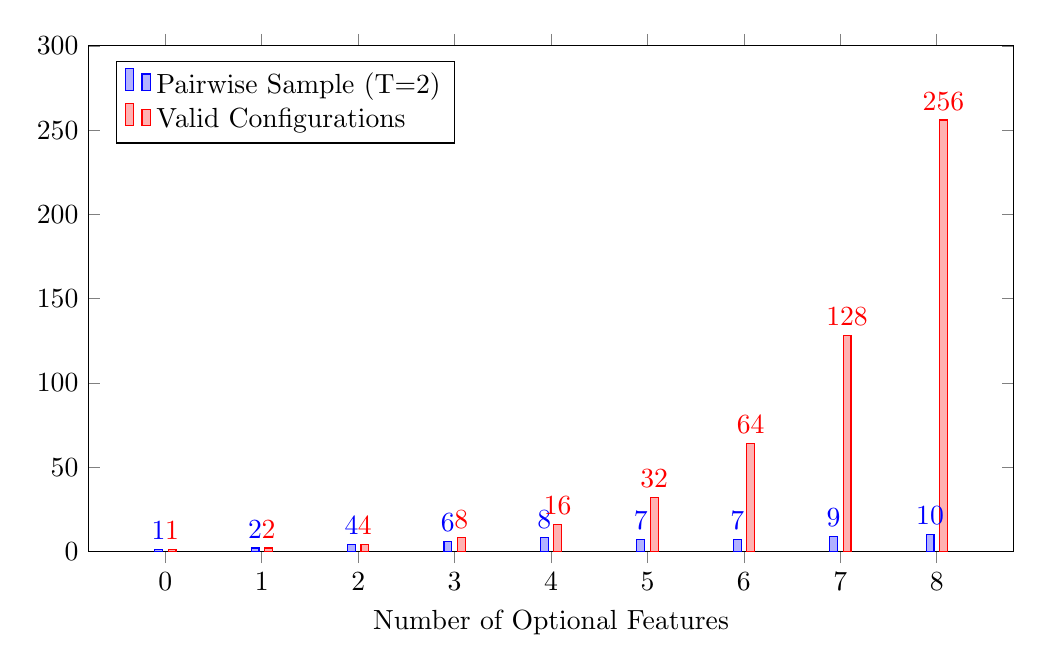
\begin{tikzpicture}
			\begin{axis}[
				width=1.1\textwidth,height=.66\textwidth,
				ybar,
				bar width=1mm,
				ymin=0,ymax=300,
				xlabel=Number of Optional Features,
				nodes near coords={\pgfmathprintnumber[precision=0]{\pgfplotspointmeta}},
				y label style={overlay},
				legend style={at={(0.03,0.97)},anchor=north west,fill=none},
				legend cell align=left,
				]
				\addplot coordinates {(0,1) (1,2) (2,4) (3,6) (4,8) (5,7) (6,7) (7,9) (8,10)};
				\addplot coordinates {(0,1) (1,2) (2,4) (3,8) (4,16) (5,32) (6,64) (7,128) (8,256)};
				\legend{Pairwise Sample (T=2),Valid Configurations}
			\end{axis}
		\end{tikzpicture}
	\end{exampletight}
	\nextcolumn
	\begin{exampletight}{Assumption: All Features are Optional}
		\centering\pic[width=.66\textwidth]{productlines/optional-features}
	\end{exampletight}
	
	\begin{exampletight}{Number of Configurations in T-Wise Sample}
		\footnotesize\centering
		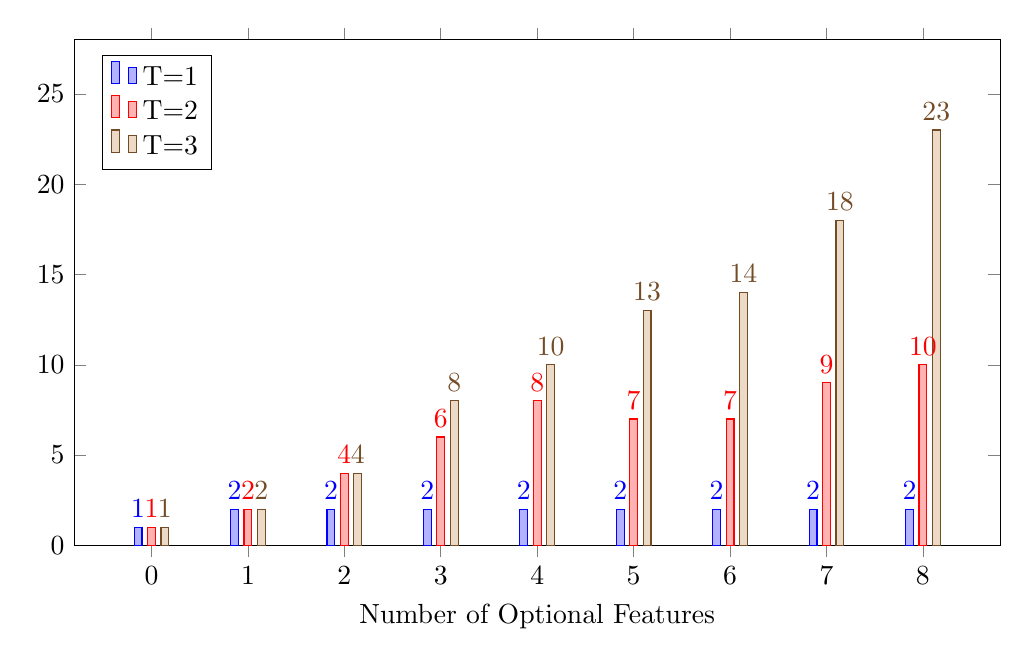
\begin{tikzpicture}
			\begin{axis}[
				width=1.1\textwidth,height=.66\textwidth,
				ybar,
				bar width=1mm,
				ymin=0,ymax=28,
				xlabel=Number of Optional Features,
				nodes near coords={\pgfmathprintnumber[precision=0]{\pgfplotspointmeta}},
				y label style={overlay},
				legend style={at={(0.03,0.97)},anchor=north west,fill=none},
				legend cell align=left,
				]
				\addplot coordinates {(0,1) (1,2) (2,2) (3,2) (4,2) (5,2) (6,2) (7,2) (8,2)};
				\addplot coordinates {(0,1) (1,2) (2,4) (3,6) (4,8) (5,7) (6,7) (7,9) (8,10)};
				\addplot coordinates {(0,1) (1,2) (2,4) (3,8) (4,10) (5,13) (6,14) (7,18) (8,23)};
				\legend{T=1,T=2,T=3}
			\end{axis}
		\end{tikzpicture}
	\end{exampletight}
\end{fancycolumns}
\end{frame}

\begin{frame}{Recap on Lecture 12: Automotive Software} % copied from se2-12b
	\begin{fancycolumns}[columns=3,widths={5,90,5},animation=none]
		\nextcolumn
		\myexampletight{}{\centering\pic[width=\linewidth]{automotive/centralized_architecture}}
		\uncover<2->{\mynote{}{redundancy still needed for the fail safe mode}}
		\nextcolumn
	\end{fancycolumns}
\end{frame}

\subsection{Exam Preparation}
\begin{frame}{\insertsubsection}
	\begin{fancycolumns}[widths={45}]
		\begin{definition}{Exam Facts}
			\begin{itemize}
				\item written exam, 90 minutes
				\item typically 80 points
				\item idea: about 1 point per minute
				\item buffer: about 10 minutes
				\item 7 tasks with about 10--15 points each
			\end{itemize}
		\end{definition}
	\nextcolumn
		\begin{definition}{Tentative Exam Structure}
			\begin{enumerate}
				\item Multiple Choice (incl. guest lectures)
				\item Evolution and Maintenance
				\item Design Patterns
				\item Compilation and Static Analysis
				\item Dynamic Analysis and Configuration Management
				\item Design by Contract and Open-Source Software
				\item Software Product Lines and Automotive Software
			\end{enumerate}
		\end{definition}
	\end{fancycolumns}
\end{frame}

